\documentclass[journal, letterpaper]{IEEEtran}
\usepackage{lipsum}
\usepackage{titlesec}
\usepackage[table]{xcolor}
\usepackage{makecell}
\usepackage[most]{tcolorbox}
\usepackage{graphicx}


\titleformat{\section}
    {\centering\normalfont\Large\bfseries}
    {}
    {} 
    {}

\newtcolorbox{theory}[2][]{breakable,sharp corners, skin=enhancedmiddle jigsaw,
parbox=false, boxrule=0mm, leftrule=2mm, boxsep=0mm, arc=0mm, outer arc=0mm,
attach title to upper, after title={\ },
coltitle=black, coltext=black,
colback=blue!10, colframe=blue!50,
title={#2}, fonttitle=\bfseries, #1}

\newtcolorbox{example}[2][]{breakable,sharp corners, skin=enhancedmiddle jigsaw,
parbox=false, boxrule=0mm, leftrule=2mm, boxsep=0mm, arc=0mm, outer arc=0mm,
attach title to upper, after title={\ },
coltitle=black, coltext=black,
colback=gray!10, colframe=gray!50,
title={#2}, fonttitle=\bfseries, #1}

\newtcolorbox{aside}[2][]{breakable,sharp corners, skin=enhancedmiddle jigsaw,
parbox=false, boxrule=0mm, leftrule=2mm, boxsep=0mm, arc=0mm, outer arc=0mm,
attach title to upper, after title={\ },
coltitle=black, coltext=black,
colback=red!10, colframe=red!50,
title={#2}, fonttitle=\bfseries, #1}


\title{COMP3131 Notes}
\author{Ronnie Low}
\date{Term 1, 2026}

\begin{document}

\maketitle

\begin{theory}{Compiler components}\\
    What are the parts of a compiler to generate machine code?
    \begin{itemize}
        \item Scanner - reads text \& produces tokens
        \item *Recogniser - reads tokens and checks for syntax errors
        \item Parser - builds abstract syntax tree (AST)
        \item Static Semantics - checks semantics at compile time 
        \item Code Generator - generates Java bytecode
    \end{itemize}
    $_{*the\ recogniser\ is\ part\ of\ the\ parser}$
\end{theory}

\begin{example}{Assessment}\\
    What is this silly marking scheme lol\\
    \\
    \begin{tabular}{ c c c }
        Component & Marks & Due\\
        Scanner & 12 & w2\\
        Recogniser & 12 & w3/4 \\
        Parser & 18 & w5 \\
        Static Semantics & 30 & w8\\
        Code Generator & 28 & w10\\
        Final & 100 & Apr/May\\
    \end{tabular}
\end{example}

\begin{theory}{What is a Compiler?}\\
    Compilers aim to:
    \begin{itemize}
        \item recognise legal and illegal programs
        \item generate correct (hopefully efficient) code
    \end{itemize}
\end{theory}

\begin{theory}{What is Lexical Analysis?}\\
    Lexical analysis is conducted by scanners. It converts code into tokens!\\
    Tokens are the basic unit of syntax; consider:
    $$position = initial + rate * 60$$
    In this case, this is broken down to:
    \begin{itemize}
        \item identifier "position"
        \item assigment operator $=$
        \item identifier "initial"
        \item plus sign
        \item identifer "rate"
        \item multiplication sign
        \item int const $60$
    \end{itemize}

\end{theory}

\begin{theory}{What is Syntax Analysis}\\
    A parser conducts syntax analysis.
    Lets consider the aim of syntactic analysis:
    \begin{itemize}
        \item groups tokens into grammatical phrases
        \item represents the graphical phases as an AST
        \item produces meaningful error messages
        \item attempts error detection and recovery
    \end{itemize}

    Syntactic analysis groups tokens into a selected format specified by a CFG
    (context-free grammar)\\
    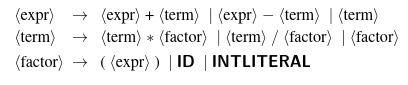
\includegraphics[width=\textwidth]{img/cfg-example1.png}
\end{theory}

\begin{theory}{What is Semantic Analysis}\\
    So whats the difference between syntax and semantic analysis?\\

    Examples of semnatic errors are:
    \begin{itemize}
        \item variables before definition 
        \item operands with incomplete types
        \item procedures (fn) called with right number and types of arguments
    \end{itemize}

    Semantic analysis also conducts type checking! 
    \begin{itemize}
        \item Floats shouldn't be used to index an array
        \item type conversions must be valid (String to class isnt valid!)
        \item for instance, 1 in binary is 0b1. 1.0 in binary is
            0b00111111100000000000000000000000. The conversion needs to be correct!
    \end{itemize}
\end{theory}

\begin{theory}{What is Code Generation?}\\
    Code generation creates an explicit IR. In our case, it generates it into Java
    Bytecode! Generally, its the process of converting your AST into executable code -
    that can be binary, bytecode or something else!
\end{theory}

\begin{aside}{Errors, Reporting \& Recovery}\\
    Consider our types of detection:
    \begin{itemize}
        \item lexical errors -> "123" as an unterminated string or something that can't be
        tokenized
        \item syntax errors -> No closing parenthesis, no semicolon
        \item semantic errors -> invalid type/number of operands for an operator
    \end{itemize}

    We want these errors to be reported as accurately (the location) as possible,
    alongside the type of error. After detecting the error, we can choose to recover and
    proceed, allowing more errors to be detected.
\end{aside}

\begin{example}{Tokens \& Lexmes}\\
    Tokens are the conversion of code into an abstract symbol used by the compiler that
    represents a lexical unit. A lexical unit is something that is predetermined by the
    compiler to be "something" that it understands. For instance, it could be a function
    call, variable, expressions, or even just a symbol ($+$)!

    Lexmes are a field within a token that specifies its name! This can be used for
    debugging purposes. Imagine this piece of code:
    $$int\ var = 8;$$
    tokenising our line results in: $[int, var, =, 8, ;]$. These are the lexmes of the
    token (the given names). Under the hood, the compiler will then assign these tokens
    certain types with patterns to make it more digestible for the compiler.
\end{example}

\begin{theory}{Patterns}\\
    Patterns are rules that describe the set of lexemes that can represent a particular
    token. As such, the pattern needs to match each string in the set.\\

    Patterns are used to convert your lexemes into token types!
\end{theory}

\begin{example}{Regex, pattern matching}
    We need a way to formally specify patterns! For instance, we need a way to match your
    lexeme as a token!\\
    Lets take an integer as example:
    \begin{itemize}
        \item intLiteral: digit (digit)*
        \item digit: $0\|1\|...\|9$
    \end{itemize}
    Lets take a float as example:
    \begin{itemize}
        \item floatLiteral: $digit* fraction\ exponent?$
                $|\ digit+$
                $|\ digit+.exponent$
        \item digit: $0\|1\|...\|9$ 
        \item fraction: $.digit+$
        \item exponent: $(E|e)(+|-)?digit+$
    \end{itemize}
    Lets decode this: $?$ implies optional. This means that:
    \begin{itemize}
        \item e+1
        \item E8
        \item e-22
    \end{itemize}
    are all valid!
    $*$ implies the prev item can repeat $0..n$ times!
    $+$ implies the prev item can repeat $1..n$ times!
    $|$ is OR - $a|b$ means pick between a OR b, but not both
\end{example}

\begin{aside}{How are tokens represented?}\\
    the 3131 compiler represents tokens as an object. I like to think of it better as a
    struct. It just a thing that holds metadata about each delimited item in the code!\\

    In VC, tokens have a enum type (intliteral, PLUS SIGN, comma, ID for variables), a
    lexeme, the column start and end of the token as well as the line number!
\end{aside}

\begin{example}{Finite State Machines}\\
    You can also use finite state machines to describe patterns!\\
    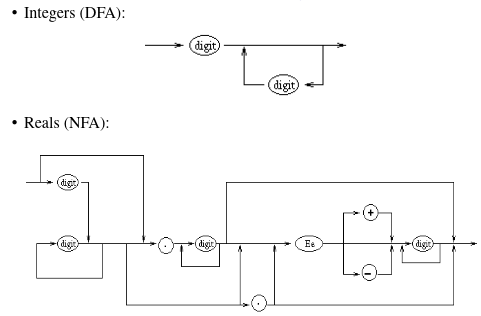
\includegraphics[width=\textwidth]{img/fsm-example1.png}
\end{example}

\begin{example}{Scanners \& longest possible matches}\\
    Scanners want to create the longest possible match: Take the token $>=$ for example:
    \begin{itemize}
        \item we do not want our scanner to yield the two tokens: ${>, =}$ (even if it is
            correct)
        \item we want our scanner to tokenize greedily - it should instead form $>=$ as a
            token even after seeing $>$ being a valid token, and only terminate on failing
            pattern matches
        \item what about failing pattern matches?
    \end{itemize}\\
    It is not the scanner's job to solve syntax errors. $12.0e+ 32$ is invalid syntax, but
    it is not our job (at least the scanner's!) to say that this is incorrect.
    Instead, the scanner will try its best to create the longest possible match, tokenising:

    $$12.0 = float$$
    $$e = id\ (var)$$
    $$+ = PLUS$$ 
    $$32 = INTLITERAL$$
\end{example}

\begin{aside}{lexical errors}\\
    Lexical errors are few and far between - these are ??? someone explain
    examples of lexical errors are:
    \begin{itemize}
        \item unterminated comment (/*)
        \item error tokens: (\%)
        \item unterminated string
        \item illegal escape character
    \end{itemize}
\end{aside}

\begin{aside}{Syntax and Semantics (langauge)} \\
    \begin{enumerate}
        \item John eats apples
        \item apples eat john
    \end{enumerate}

    Syntax is only concerened with the form/structure of english sentences and its grammar
    Semantics is concered with the meaning of the sentence
\end{aside}

\begin{theory}{Syntax and Semantics (Progrmaming languages)}\\
    \begin{itemize}
        \item syntax refers to the form/structure of programs
        \begin{itemize}
            \item no concern with the meaning of programs
            \item specificed by a context free grammar
        \end{itemize}
    \item semantics refer to two notions:
        \begin{itemize}
            \item Static semantics refer to restrictions enforced at compile time 
                \begin{itemize}
                    \item all identifiers (variables) are declared before used 
                    \item assignment must be type compatible (int identifier cannot be
                        equals to a string)
                    \item operands must be type compatible
                    \item 
                \end{itemize}
            \item runtime semantics refer to what the program does/computes
                // TODO: fill ts out
        \end{itemize}
    \end{itemize}
\end{theory}

\begin{example}{Static semantics}\\
    ```i = 5;``` 
    Syntactically, this is fine. But we have not declared the variable `i` beforehand.
\end{example}

\begin{aside}{Semantic analyser and semantic errors}\\
    aside
\end{aside}

\begin{theory}{Context Free Grammar}\\
    used to specify language's syntax 
    simple 
    regular grammars
\end{theory}

\begin{theory}{CFG's formal definitions}\\
    grammar is a quadruple $(V_T, V_N, S, P)$
    $V_T$ -> finite set of terminal symbols (tokens)
    $V_N$ -> finite set of nonterminal symbols
    $S$ -> unique start symbol 
    $P$ -> finite set of rules 
\end{theory}

\begin{example}{Leftmost \& rightmost derivations} \\
    example
\end{example}

\begin{theory}{What is a language} \\
    langauge is defined by a grammar : all the sentences derived from a grammar.

\end{theory}

\begin{theory}{How do we specify a cfg}\\
    BNF
\end{theory}

\begin{theory}{How do we derive if somethign is syntacially correct}\\
    build a parse tree
\end{theory}

\begin{aside}{Grammar summary}\\
    how langauge is defined with CFG
    syntax and semantics
    precednece and associativity of grammar
    CFG has four components
    parsing: check for syntax errors and construct AST
\end{aside}

\begin{example}{EBNF}\\
    example
\end{example}
    
\end{document}
